\subsection{Interpretability}
Previous work by the authors \cite{hyett2022applicability} suggested there may be a latent space in the invariants when predicting the PH using the TBNN. The existence of a latent space could be important to the ability to interpret the results, e.g. searching for a functional form or providing physical insight; or if we believe in the statistical independence of the input (in our case there are many reasons to) it suggests the network struggles to exploit the additional information. In the case of \cite{hyett2022applicability} it seems to be the latter.

The proposed latent space is indeed persistent when training the network having normalized the PH using $\tau^2$, in particular, the latent space claimed consists only of the low-order invariants. The hypothesis by the author was that the latent space emerged as a numerical artifact of strong normalization of the high-order invariants ($\lambda_{3,4} \to \tau^3 \lambda_{3,4}$, and $\lambda_5 \to \tau^4 \lambda_5$). But as we show in figure(\ref{fig:dg}), there exists leading-order sensitivity to $\lambda_5$ (and not insignficant sensitivity to $\lambda_{3,4}$) when the PH is \textit{not} normalized. This may indicate that the low-order latent space was a numerical artifact resulting from very small weights in the \textit{output layer}, combined with strong normalization of high-order invariants.

\begin{figure}
    \centering
    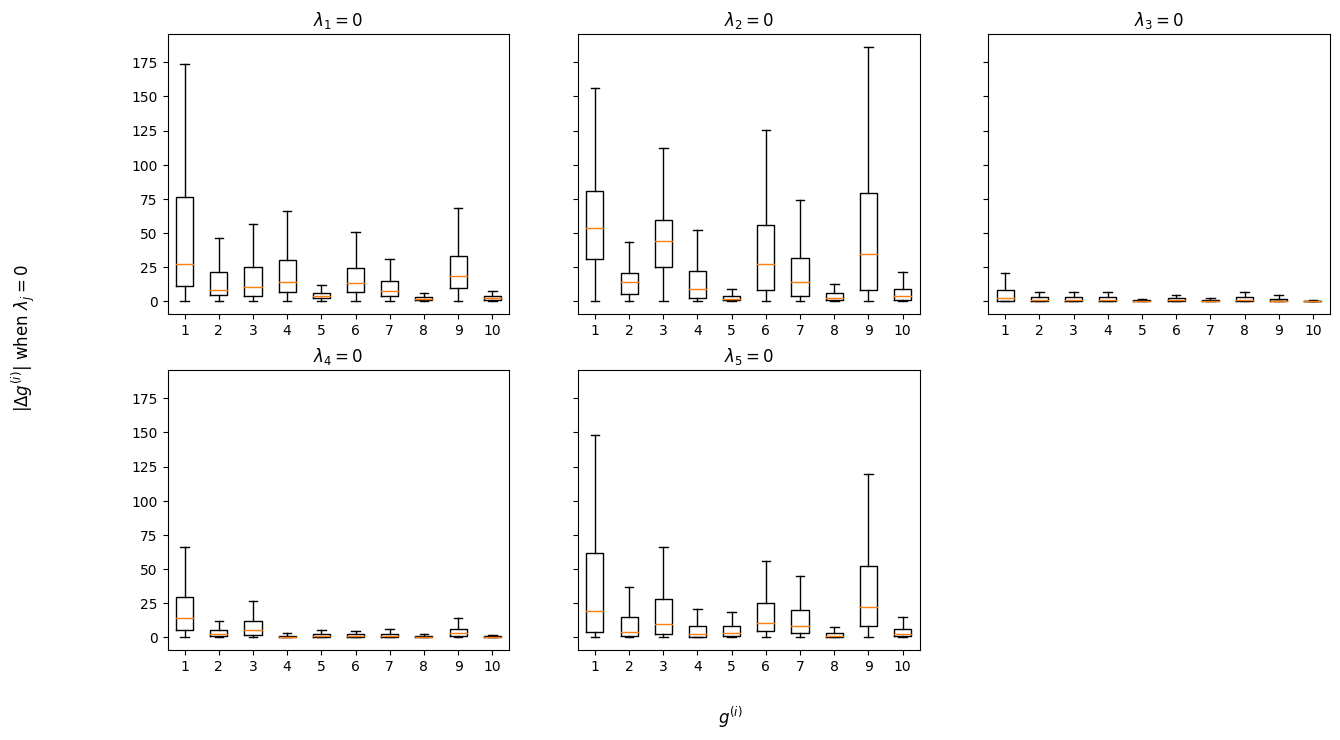
\includegraphics[width=\textwidth]{LagrangianDeformationModels/figs/dg.png}
    \caption{Distributions of sensitivity of $g^{(i)}$ to variability of $\lambda_j$. Previous work performed suggested that $\lambda_{3-5}$ were unimportant to the prediction using the TBNN. This result was predicated upon the normalization of the PH using $\tau^2$. While our plot reinforces that $\lambda_{3,4}$ do provide an order of magnitude smaller correction, the sensitivity of the network to $\lambda_5$ is of the same order of magnitude as that to $\lambda_{1,2}$. This suggests that by \textit{not} normalizing the PH, we are able to exploit additional information in the invariants.}
    \label{fig:dg}
\end{figure}

To explore this question further, we applied an autoencoder to the set of invariants, as well as calculated the mutual information between the invariants.

The mutual information calculation, shown in table(\ref{tab:mutualInformation}), indicates that while the invariants are not strictly independent, they are also far from highly correlated. The maximum value - biased away from the ideal value of $10$ here by the k-nearest neighbors algorithm with $k=5$, detailed in \cite{ross2014mutual}.
\begin{table}
\centering
\begin{tabular}{|c|c|c|c|c|c|}
  \hline
  $I(\lambda_i, \lambda_j)$ & $\lambda_1$ & $\lambda_2$ & $\lambda_3$ & $\lambda_4$ & $\lambda_5$\\
  \hline
  $\lambda_1$ & & 0.26350727 & 1.40593169 & 0.40473788 & 0.72127464\\
  \hline
  $\lambda_2$ & & & 0.1968969 &  0.80102301 & 0.95679744\\
  \hline
  $\lambda_3$ &  &  & & 0.43549834 & 0.49519878\\
  \hline
  $\lambda_4$ & & & & & 0.83990126\\
  \hline
  $\lambda_5$ & & & & & \\
  \hline
\end{tabular}
  \caption{A scaled mutual information $I(\lambda_i, \lambda_j)$, between invariants. Note the maximum value is near $10$, the method used here introduces a bias however, namely via k-nearest neighbors with $k=5$, as discussed in \cite{ross2014mutual}}
    \label{tab:mutualInformation}
\end{table} 

\begin{figure}
    \centering
    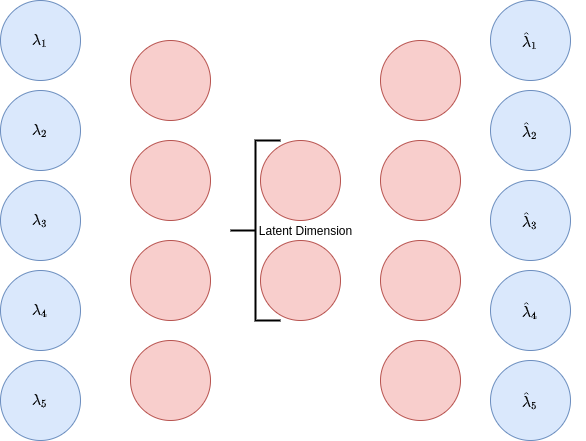
\includegraphics[width=0.5\textwidth]{InterpretableML/figs/aeStructure.png}
    \caption{Autoencoder structure applied to the invariant input data.}
    \label{fig:aeStructure}
\end{figure}

The autoencoder structure is a fully connected, feed forward neural network, 
\begin{equation}
    AE_\theta: \R^5 \to \R^5 \text{ via } \R^5 \to \R^4 \to \R^h \to \R^4 \to \R^5
\end{equation}
where $h$ is the imposed latent dimension, illustrated in fig[\ref{fig:aeStructure}]. The nonlinear activation functions of $AE_\theta$ are the so-called "leaky-relu". We implement the "robust max-min" normalization, relying on the interquartile distance - namely, letting $Q_1, Q_3$ be the first and third quartiles, we normalize our invariants as
\begin{equation}
    \Tilde{\lambda_i} = \frac{\lambda - Q_1}{Q_3 - Q_1}
\end{equation}
This is intentionally different than the normalization used in the TBNN, as normalizing via timescale and optimizing using the mean-squared-error gives a very strong preference towards reconstructing only the low-order invariants. The robust max-min normalization is an attempt to set each on an equal footing, but itself is subject to biases introduced by differences in distribution shapes.

We use the ADAM optimizer with learning rate $\eta = 1e-3$, partitioning the dataset of 100k samples into 75\% training, 25\% test. The results are shown in fig[\ref{fig:aeLoss}] and may suggest a small reduction in dimension (i.e., $5\to 3$). These results match the leading order contributions to the sensitivities of the $g^{(i)}$ as shown in fig(\ref{fig:dg}), but we caution this suggestion as the low-order basis elements are still significantly influenced.
\begin{figure}
    \centering
    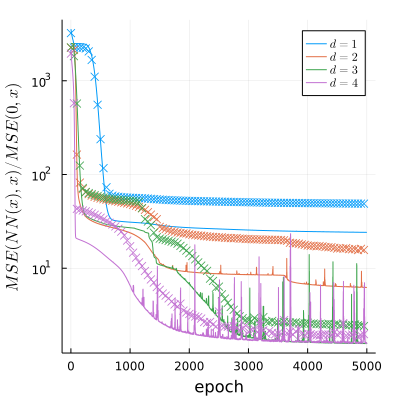
\includegraphics[width=\textwidth]{InterpretableML/figs/aeInvariants.png}
    \caption{Autoencoder applied to the invariant input data, in an attempt for a nonlinear projection onto a latent space. (Left) shows the evolution of the loss according to the imposed latent dimension, where 'x's mark test loss, while solid lines mark training loss. (Right) shows the minimum loss as a function of latent dimension. Notice the two jumps at $h = 2$ and $h=3$ - suggesting a sequence of increasing fidelity.}
    \label{fig:aeLoss}
\end{figure}
